\documentclass[letter:wpaper]{article}
\usepackage{isea}
% UPDATE: See the local /.vscode/settings.json
% The pdftex option is necessary for the pdfinfo command to work, for the graphicx package to work, and for the correct fonts to work. It requires the pdfLaTeX renderer
% [1] Select the Preferences: Open User Settings (JSON) command in the Command Palette (⇧⌘P)
% [2] Find the latex-workshop.latex.recipes setting and move the "xelatexmk" recipe to the top of the list. This will make xelatexmk the default recipe for building LaTeX files.
%
%   "latex-workshop.latex.recipes": [
%     {
%       "name": "latexmk",
%       "tools": ["latexmk"]
%     },
%     {
%       "name": "latexmk (xelatex)",
%       "tools": ["xelatexmk"]
%     }
% [3] There is no 3. There is already a "latex-workshop.latex.tools" setting for "latexmk" that uses the -pdf flag and so will use pdfLaTeX. I suppose [3] is for putting xelatexmk back as the default recipe
\usepackage[pdftex]{graphicx}
\pdfinfo{
    /Title (Art as Technology)
    /Author (Kynan Stewart Hughes)
}
\usepackage{times}
\usepackage{helvet}
\usepackage{courier}
\usepackage[numbers]{natbib}
% The file isea.sty is the style file for ISEA 2025 proceedings.
%
\title{Art as Technology (v1.1.0.9)}
\author{Kynan Stewart Hughes\\
Creativity and Cognition Studios\\
University of Technology Sydney\\
Sydney, Australia\\
kynan.s.hughes@student.uts.edu.au\\
\newline
\newline
}
\setcounter{secnumdepth}{0}

\begin{document} 
% Setting the default tolerance level
% \tolerance=200
% Setting a high tolerance level
% \tolerance=10000
% Some more drastic measures for hbox issues
% \emergencystretch=4em
% \raggedright
\maketitle
\begin{abstract}
    This paper argues that art should be understood as a technology. Drawing on complexity science and Process philosophy, it frames art as a codifying system that reconfigures materials and objects to produce contextual meaning. Rethinking art in technological terms also invites a more nuanced, ethically attuned understanding of technological evolution. The author’s own artwork contributes to this argument. The paper concludes by encouraging artists working with emerging technologies to explore an attitude to crafting grounded in sensitivity to affect and the complex interdependence of things.
\end{abstract}

\keywords{Keywords}

Art, technology, complexity, aesthetics, affect, information, craft, ethics, systems, emergence, meaning, constraints, coarse–graining

-------- [SLIDE] --------

-------- [SLIDE] --------

\section{Introduction}

    This paper explores the idea that art is a technology \citep[pp.74–75]{SauvagnarguesArtmchns2016} \citep{GellThTchnlgyOfEnchntmnt1992} \citep[p.202]{OSullivanFrmAsthtcsToThAbstrctMchn2010} -- an idea that grounds art as a material practice and which also has the potential to change the way we think about technological change. 
    
    The theoretical lens is a mixture of complexity science and contemporary Process philosophy, especially Brian Massumi's concept of affect, which has redefined aesthetics in recent years, and Jacques Rancière's systemic, materialist theories of art. At one point I mention one of my own artworks as a kind of cautionary tale.

-------- [SLIDE] --------

\section{A Definition of Technology} 

-------- [SLIDE] --------

    From the perspective of Complex Adaptive System Theory, a technical object is always a phenomenon, or phenomena, ``captured and put to use.'' \citep[p.53]{theNatureOfTechnology2009}. To put it another way, technology is ``programming [...] phenomena for [...] purpose.'' \citep[p.53]{theNatureOfTechnology2009}. This is a simple and powerful distillation because it holds for all technologies, contemporary and historical, and it takes the idea of technology beyond just physical, mechanical objects.
    
    A key point is that ``phenomena'' don't have to be physical, like fire or electricity. They may be ``behavioural or organisational effects'' \citep[p.55]{theNatureOfTechnology2009}, or simply ``truism[s] of nature'' \citep[p.45]{theNatureOfTechnology2009}. Any ``perceived regularity'', in the terminology of complexity science \citep[p.2]{FlackCrsGrnngAsDwnwrdCstn2021}

-------- [SLIDE] --------

    \subsection{Example: Money}

    For example, Money is a technology.

    \begin{quote}
        The monetary system makes use of the ``phenomenon'' that we trust a medium has value as long as we believe that others trust it has value and we believe this trust will continue in the future. \citep[p.55]{theNatureOfTechnology2009}
    \end{quote}

-------- [SLIDE] --------

\section{A Definition of Art}

-------- [SLIDE] --------

    Jacques Rancière has called contemporary Western art ``the aesthetic regime'' \citep[p.23]{RancierPltcsOfThAsthtcs2004}. It is a ``regime of perception'' \citep[p.xii]{RancièreAisthesis2013}, a ``mode of thought'' that ``runs through the specific definitions that the arts have given to themselves in the Modern Age'' \citep[p.23]{RancierPltcsOfThAsthtcs2004}. It's emergence at the end of the eighteenth century coincided with Immanuel Kant's \emph{Critique of Judgement} \citep[pp.23–24]{RancierPltcsOfThAsthtcs2004}. 

    Within the aesthetic regime, all distinctions and differences operate in relation with the idea of aesthetic experience. Styles like Modernism and Post–Modernism, for example, are simply different strategies for making aesthetic objects \citep[p213]{ZepkeSblmArt2017}. Art which is anti–aesthetic is operating within the aesthetic regime by being self–consciously critical of it\footnote{
        Reference.
    }. Conceptual art is art that invites us to consider the aesthetic potential of ideas\footnote{
        Reference.
    } -- and so on.

    Art in this sense is a complex codifying system that dislocates objects from their original functions and meanings and gives them new functions and meanings. The ``dissensual operation'' \citep[p.54]{RancierThEmncptdSpcttr2009} of creating an artwork, for example by working a material into a form, or by setting the state of pixels on a screen, or by appropriating a ready–made object, literally ``transforms a given form or body into a new one.'' \citep[p.54]{RancierThEmncptdSpcttr2009}.

-------- [SLIDE] --------

\section{Affect}

The concept of \emph{affect}, which comes from Deleuze and Guattari via Brian Massumi, is a way of thinking about how things affect other things in complex systems of interconnections that is the world. It is the way that we and things are moved by the world and each other. When it happens in humans, it is a kind of pre-cognitive, pre-linguistic, pre-conscious event during which the world emerges into existence. 

Affect is when emergence happens. It’s a moment of quantum indeterminacy “fed forward” across levels of reality \citep[p.37]{MassumiPrblsFrThVrtl2002} until it may register as cause and effect. In turn, this apparent causality feeds back as “downward causation” \citep[p.?]{FlackCrsGrnng2017}, influencing the behaviour of system components. Affective exchanges are ongoing at every level of organisation.

Humans are especially tuned to affective regularities \citep{FristonThFrEnrgPrncpl2010, DeaconTheSymbolicSpecies1998}. We notice patterns: the rhythm of seasons, animal behaviours, music, language. These patterns help us make sense of the world.

Art, under the aesthetic regime, exploits this sensitivity. It’s a codifying system — a hack — that charges objects with affect, like a battery.

The shift from beauty to affect reframes aesthetic experience as material and emergent. Art is now about “complex affective and intensive exchanges, situated in the broader ecology of the world.” \citep[p.155]{HighmoreBttrAftrTst2010}

The affective charge of an artwork can include qualities that are—

-------- [SLIDE] --------

strong,

-------- [SLIDE] --------

gentle,

-------- [SLIDE] --------

sensorial,

-------- [SLIDE] --------

semantic,

-------- [SLIDE] --------

abstract,

-------- [SLIDE] --------

pleasant and

-------- [SLIDE] --------

unpleasant.

-------- [SLIDE] --------

It may strobe between incompatible states — like the cute and the grotesque.

\section{Purpose}

    -------- [SLIDE] --------

    According to Felix Guattari, art ``confers a function of sense and alterity to a subset of the perceived world'' \citep[p.131]{GuattariChsmss1995}. In other words, an artwork is \emph{about} something.

    Arthur Danto described art as ``embodied meaning'' \citep[p.125]{DantoEmbdMnngs2007} -— a useful framing, so long as we remember that meaning is always contextual\footnote{
        Manuel DeLanda notes that “meaning” in the sense of a word differs from “meaning” in the sense of a life \citep[pp.40–41]{DeLandaCsltyAndMnng2018}. Carroll’s critique of Danto assumes the former.
    }. ``Meaning is [...] a network of enveloped material processes. A thing has as many meanings as there are forces capable of seizing it.'' \citep[p.10]{MassumiAUsrsGdTCptlsmAndSchzphrn1992}

    So we arrive at an art object as a technical object: a phenomenon (our capacity to attribute affect) captured and put to use.

    -------- [SLIDE] --------

    But purpose has long distinguished art from other forms of making. For Kant, beauty was ``purposive without a purpose'' \citep[p.57]{KantCrtqOfJdgmnt} -— art’s value lay in its disinterest, its refusal of function.

    This idea persists, circular as it is. It only makes sense if one assumes art must differ fundamentally from other crafts. But from a complexity perspective, no purpose is fixed or independent —- everything is contextual.

    -------- [SLIDE] --------

    Art objects often have multiple purposes. A painting can evoke beauty (its ``art purpose'', we might say), but can also confer status, act as capital, or start a revolution. Just as artworks are indeterminate with respect to meaning\footnote{
        Hoelscher.
    }, they are indeterminate with respect to purpose.

    -------- [SLIDE] --------

    Some artworks incorporate non-art purposes into their embodied meaning without their meaning ever being reducible to them. There is always ``contextual excess or remainder'' \citep[p.252]{MassumiPrblsFrThVrtl2002}. In craft or socially connected artworks, these entanglements are deliberate.

    When art and non-art purposes mix, the art purpose can suffer —- especially in artworks made with emerging technologies, where the meanings are not yet well understood.

    -------- [SLIDE] --------

	% In the early 2000s, practitioners of locative art were criticised for their uncritical use of mapping and networked, location-aware, mobile technologies, as well as for their collaborations with industry. It was alleged that they lacked a structure of accountability and ethics, were ushering in a `society of control', and were turning the media-art conference circuit into a `shopping-driven [...] spectacle' \citep[p.358]{beyondLocativeMedia2006}. Locative art was described as a ``technocentric fantasy'' that ``downplays [...] history'' \citep[para. 2]{questioningTheFrame2004}.

    In the early 2000s, locative art drew criticism for uncritical adoption of mobile and networked technologies. Critics saw ethical blind spots, commercial entanglements, and complicity with surveillance culture \citep[p.358]{beyondLocativeMedia2006} \citep[para. 2]{questioningTheFrame2004}.

    The imagined non-art potentials of locative technologies disrupted the art-purpose of the artworks. These critiques seem valid, now that techno-capitalism and mass surveillance have become obvious realities.

    Should an artwork’s purpose becomes reducable to it's non-art purpose, it is no longer art.

    -------- [SLIDE] --------

    \subsubsection{Example: \emph{FlowAttractor}}

    \begin{figure}[h]
        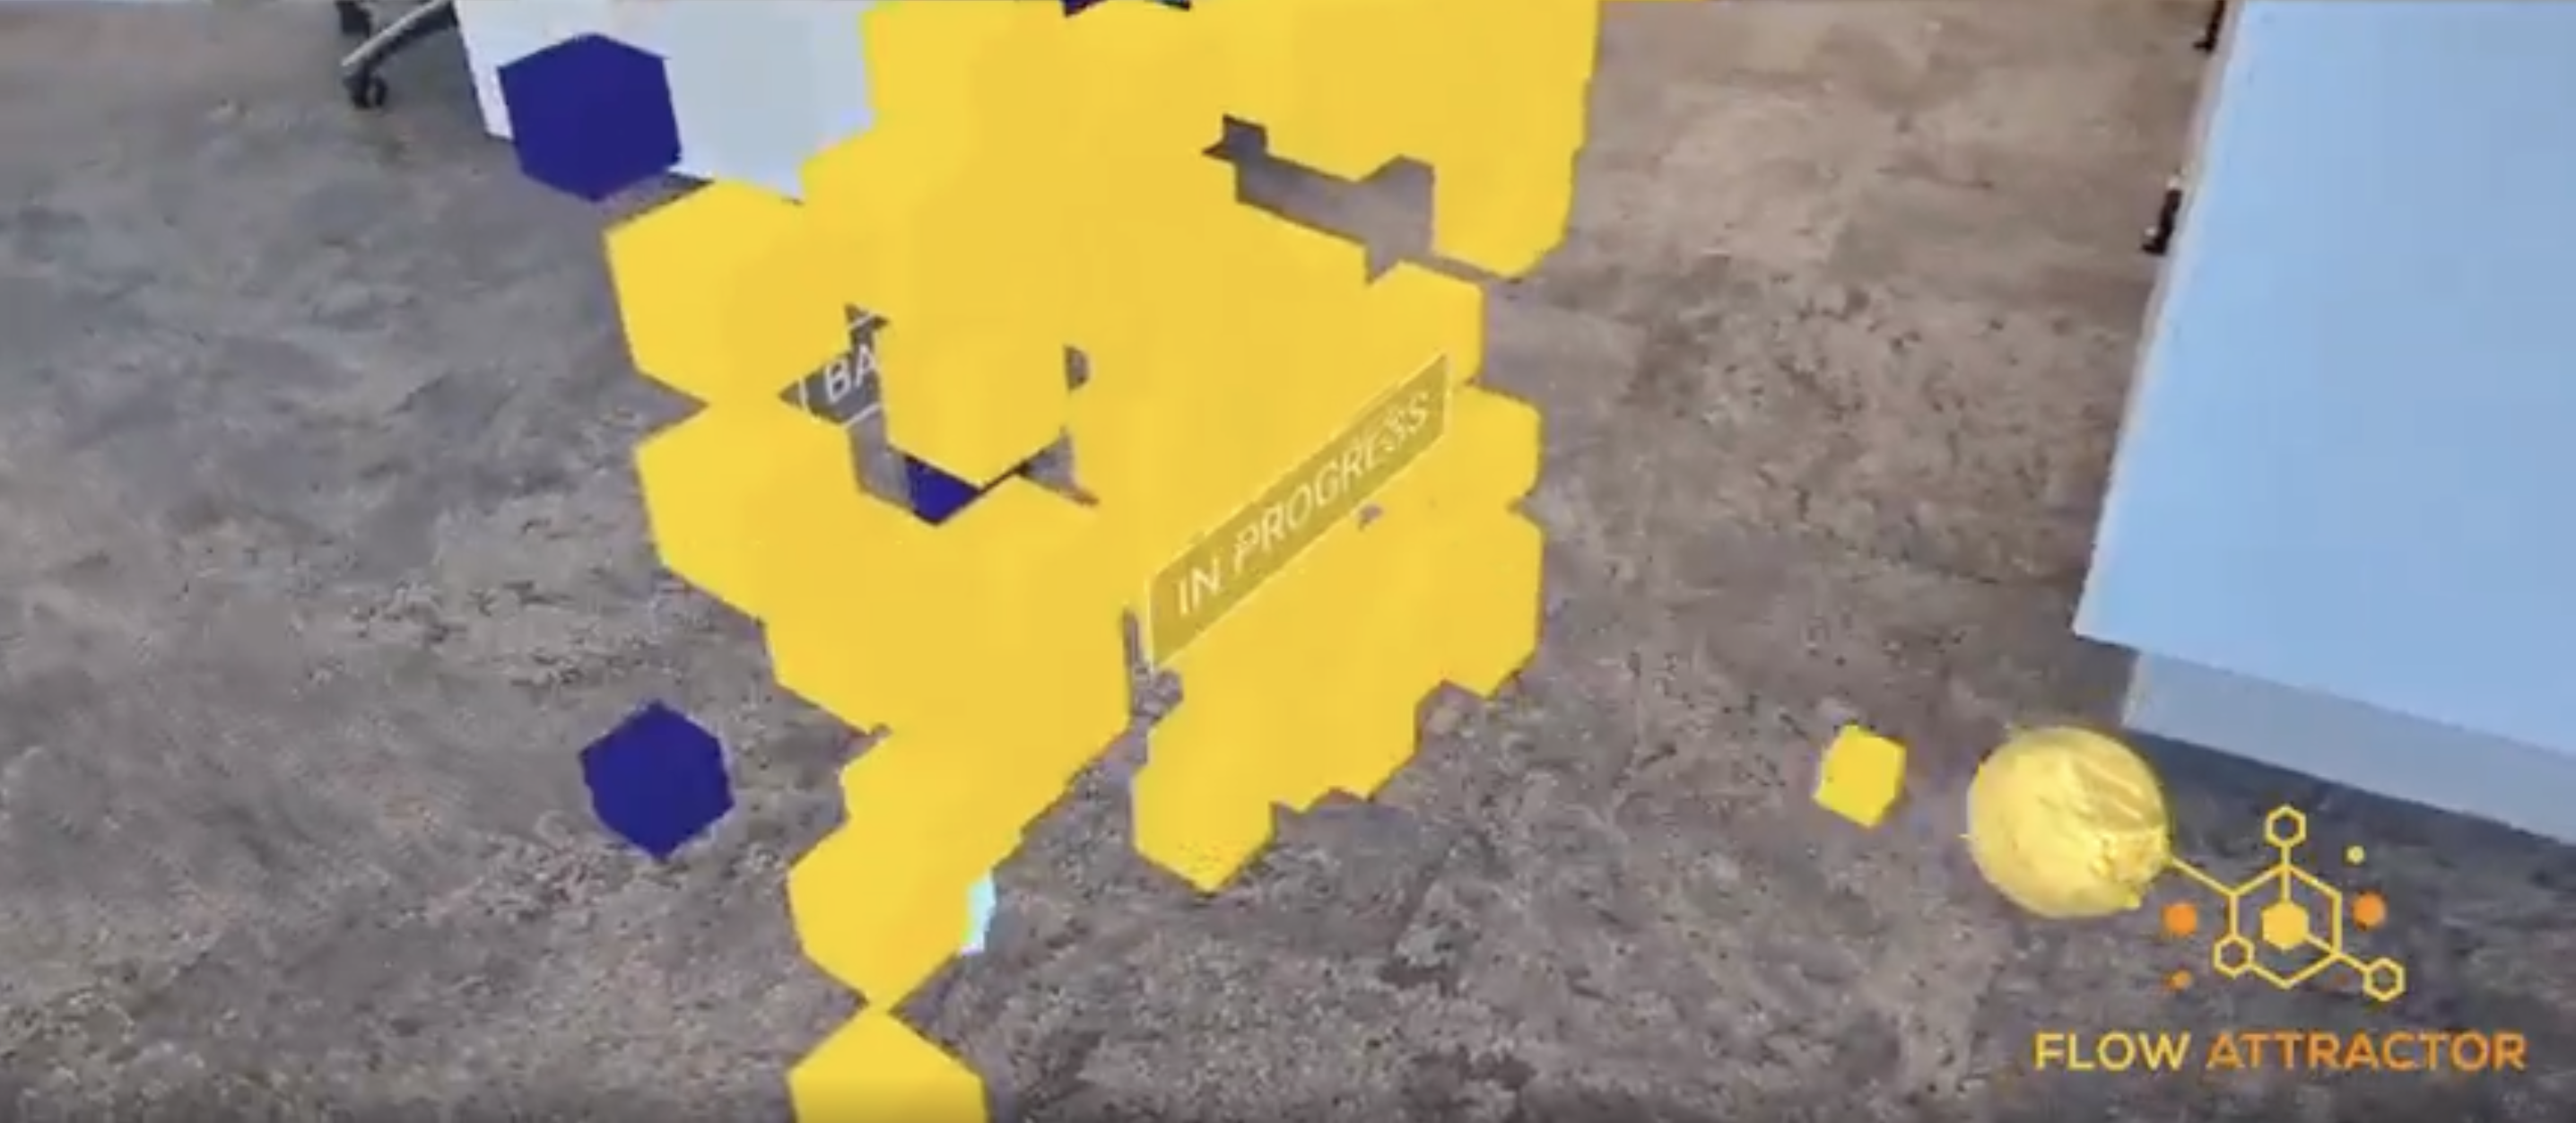
\includegraphics[width=3.31in]{flow-attractor.png}
        \caption{\emph{FlowAttractor} models complex workflows as flying cubes. \copyright Respect Copyright.}
        \label{fig:flow-attractor}
    \end{figure}

    In \emph{FlowAttractor} (Figure~\ref{fig:flow-attractor}), the flow of cubes visualises the hidden movement of work items in a bank’s software pipeline. Within that context, its purpose is to heighten awareness of small decisions that shape system flow. Augmented reality works well for this.

    But, because its meaning is completely reducible to a non–art purpose, it ceases to be an art object in that context.
    % its meaning is legible as a functional tool, its art purpose is harder to sustain. In that context, it may cease to function as art.

    -------- [SLIDE] --------

    Art’s purpose is complex, shifting, and relational. But this isn’t unique to art.

    Non-art technical objects also have indeterminate uses. For instance, we don't know exactly how Anaesthesia works\footnote{
        See Franks (2006) or Brown et al. (2010), who note the persistent uncertainty surrounding how anaesthetics induce unconsciousness.
    }.

    -------- [SLIDE] --------

    Viagra was a treatment for angina\footnote{
        See Boolell et al. (1996), “Sildenafil...”.
    }.

    -------- [SLIDE] --------

    The internet was a Cold War military network. Now it's for shrimp Jesus images, advertising, and mass surveillance.

    If art is a kind of social technology, like money, then where did we get the idea it must stand apart from all other technologies?

    Why is it strangely unthinkable to think of art as a technology?

    -------- [SLIDE] --------

\section{A Fold in the Distribution of the Sensible}
    
-------- [SLIDE] --------

    According to complexity science, ``coarse graining'' occurs when a subsystem with emergent properties is treated as a single entity by the wider system. It’s a shortcut -- like zooming out on a map to see the shape of a city, while losing the detail of its streets. It is ``lossy but true'' \citep[p.4]{FlackCrsGrnng2017}.

    Sometimes, though, it’s just lossy \citep[p.8]{FlackCrsGrnng2017}. Humans, evolutionarily tuned to find patterns, often imagine them \citep{FristonThFrEnrgPrncpl2010}.

    The perceived split between art and technology may be one such imagined pattern — a dubious piece of coarse graining that’s persisted for about six hundred years. It survives, in part, because the aesthetic regime overlays an older regime where that distinction first emerged.
    
-------- [SLIDE] --------

    \subsubsection{The Regime of Representation}

    The idea of a qualitative divide between what we now call ``the arts'' and other forms of making began to take shape during the Renaissance \citep[p.136]{TatarkiewiczWhtIsArt1971}. By the 17th century, this classification had solidified. Rancière calls this ``partitioning of the sensible'' the ``regime of representation.''\footnote{Reference.}

    The arts -- music, literature, sculpture, painting, and so on -- existed, but not as a unified category called ``art.'' They were disparate practices, each with a specific social function, nested within a hierarchical system that classified activities and people. Their collective role was to represent the world as an orderly whole -- a place for everything and everyone in their place.

    The aesthetic regime -- art as we know it -- emerged as a tactic that cut across this representational order. Yet we still observe the fold it left behind: the lingering distinction between art and other practices. We organise our schools and faculties along this line -- STEM on one side, arts and humanities on the other.

    This fold in the ``distribution of the sensible'' \citep[p.42]{RancierPltcsOfThAsthtcs2004} is what the idea of art as technology begins to smooth out. What would it mean for that fold not to exist? A look at the regime that preceded representation reveals just such a condition.

-------- [SLIDE] --------

    \subsection{The Ethical Regime of Images}

    Heidegger, in ``The Question Concerning Technology,'' noted that ``techne'' was the ancient Greek word for skill, craft, and technique — a term that covered the arts, sciences, and technical practices like sword-making and shipbuilding \citep[p.34]{HeideggerThQstnCncrngTchnlgy1954}.

    Rancière has called this worldview the ``ethical regime of images,'' where ``image'' implies that all crafted things reflect ideal forms.
    
    In this regime, ethics mattered. The ``end or purpose'' of an object — what it did in the world, how its effects shaped the ``ethos,'' the collective mode of being of individuals and communities  — was central. \citep[pp.20--21]{RancierPltcsOfThAsthtcs2004}
    
    Plato distinguished between ``true arts,'' which imitated ideal forms with clear ends, and ``lesser arts,'' which merely mimicked appearances \citep[p.20]{RancierPltcsOfThAsthtcs2004}. While these ideas now seem quaint, they formed an ethical framework linking making with consequence.
    
    Like the regime of representation, the ethical regime still lingers as a cultural substrate. We still care who makes what — and why — especially in art.
    
    -------- [SLIDE] --------
    
    In 2021, an art festival in Hobart planned to feature a work by Santiago Sierra involving blood donations from descendants of First Nations peoples who survived colonisation. Many argued the work sensationalised trauma to no positive effect. Rappers Tasman Keith and Briggs posted that they ``already gave enough blood'' \citep{DrkMfBld2021}. The piece was eventually pulled.
    
    Somewhere along the line, technological crafting became decoupled — in a way artmaking didn’t — from the kind of affective sensitivity that underpins both aesthetics and ethics. Technology evolves, it seems, regardless of how we feel about it.
    
    We may fear losing jobs or identity to AI, but those fears will be ignored.
     
-------- [SLIDE] --------

\section{Conclusion}

    To think of art as a technology is to think across the fold that separates art from technology, and to begin a process of smoothing out the fold. It challenges us to imagine what it would be like for this difference to not exist, potentially changing the way we think about both artmaking and technological development.
    
    The persistent difference between art and technology makes it unthinkable to think of art as a technology. But if this difference can be rethought, then perhaps it is a job for artists who work with emerging technologies. 
    
-------- [SLIDE] --------

    As artists working at the edges of technological evolution, we are invited to return humanity to an idea of crafting, guided by ethics informed by an aesthetic appreciation of the complex, interconnected nature of all things\footnote{
        This is essentially Guattari's idea of an \emph{ethico–aesthetic paradigm} \citep[p.131]{GuattariChsmss1995}, 
    }. Perhaps we will open a space in which humans can begin to learn how to evolve our technologies differently at a moment in history when our technologies are learning to relate differently with us.
    
    To paraphrase Gilbert Simondon, we may begin to think of ourselves as

    \begin{quote}
        inventors of technical and living objects. We coordinate and organise their mutual relation at the level of machines, between machines. [...] We construct the signification of the exchanges of information between machines. Our rapport with the technical object is a coupling between the living and the non–living. \citep[p.xvi]{SimondonOnThMdOfExstncOfTechnclObjcts1980}
    \end{quote}
    
\bibliographystyle{isea}
\bibliography{isea}

\section{Author Biography}

Kynan Stewart Hughes is a PhD candidate at the University of Technology Sydney. His research is at the conjunction of art and technology. He is a practising artist and has worked in the software industry for over 20 years. 

\end{document}